\documentclass[12pt]{beamer}

\usepackage{cmap}
\usepackage[english, russian]{babel}

\usetheme{metropolis}
\usepackage{appendixnumberbeamer}

\usepackage{booktabs}
\usepackage[many]{tcolorbox}

\usepackage{listings}
\lstset{basicstyle=\ttfamily\small,
	showstringspaces=false,
	breaklines=true,
	frame=lrtb,
	% numbers=left,
	extendedchars=\true,
	language=bash
}

\usepackage{xspace}
\newcommand{\themename}{\textbf{\textsc{metropolis}}\xspace}
% \setsansfont{Fira Sans Bold}

\title{Автоматизация миграции программного кода на новый набор библиотек}
% \subtitle{A modern beamer theme}
\date{\today}
\author{Артем Алексюк}
\institute{Санкт-Петербургский политехнический университет Петра Великого}
% \titlegraphic{\hfill
\includegraphics[height=1.5cm]{logo.pdf}}

\newtcolorbox{mybox}[1][]{
    width=\textwidth,
    arc=3mm,
%    auto outer arc,
    boxsep=0cm,
    toprule=1pt,
    leftrule=1pt,
    bottomrule=1pt,
    rightrule=1pt,
    colframe=white,
    boxrule=0pt,frame hidden,
    breakable,
    nobeforeafter,
    enhanced jigsaw,
    opacityframe=0.7,
    fontupper=\bfseries,
    opacityback=0.7
}

% \setbeamertemplate{blocks}[rounded][shadow=false]
% \addtobeamertemplate{block begin}{\pgfsetfillopacity{0.5}}{\pgfsetfillopacity{1}}

\begin{document}

\maketitle

\begin{frame}{Table of contents}
  \setbeamertemplate{section in toc}[sections numbered]
  \tableofcontents[hideallsubsections]
\end{frame}

% \section{Introduction}


{
\usebackgroundtemplate{%
\tikz\node[opacity=0.4]{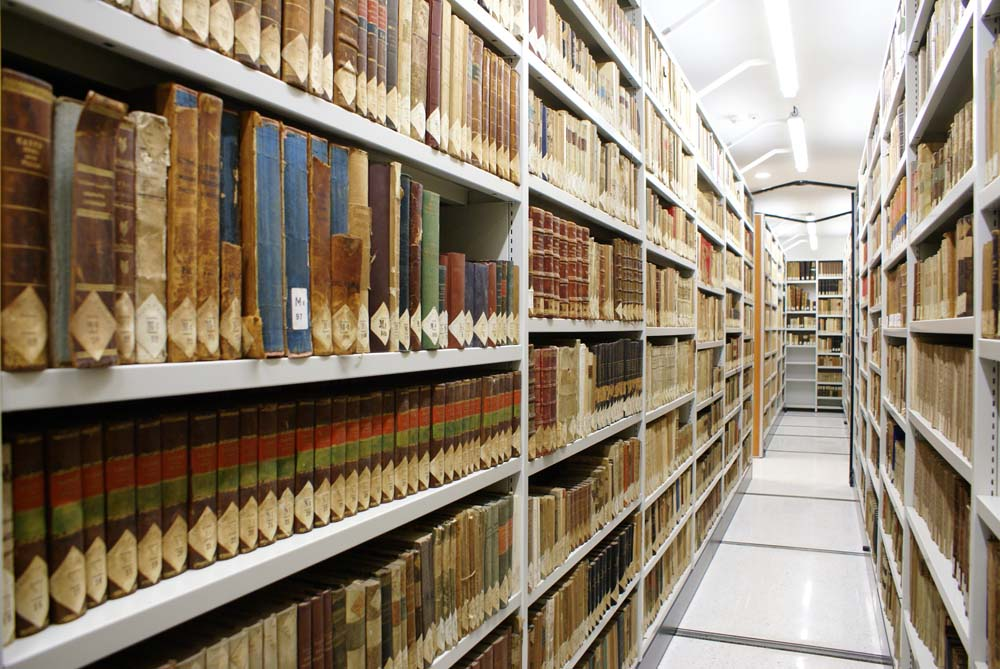
\includegraphics[height=\paperheight,width=\paperwidth]{historical-archive.jpg}};}
\begin{frame}{Актуальность}
\begin{mybox}[]
Миграция в новое библиотечное окружение?
\begin{itemize}
	\item Новая программная платформа
	\item Новая аппаратная платформа
	\item Унаследованный код, несовместимый с современными системами, средствами разработки, библиотеками
\end{itemize}
\end{mybox}
\end{frame}
}

{
\usebackgroundtemplate{%
\tikz\node[opacity=0.4]{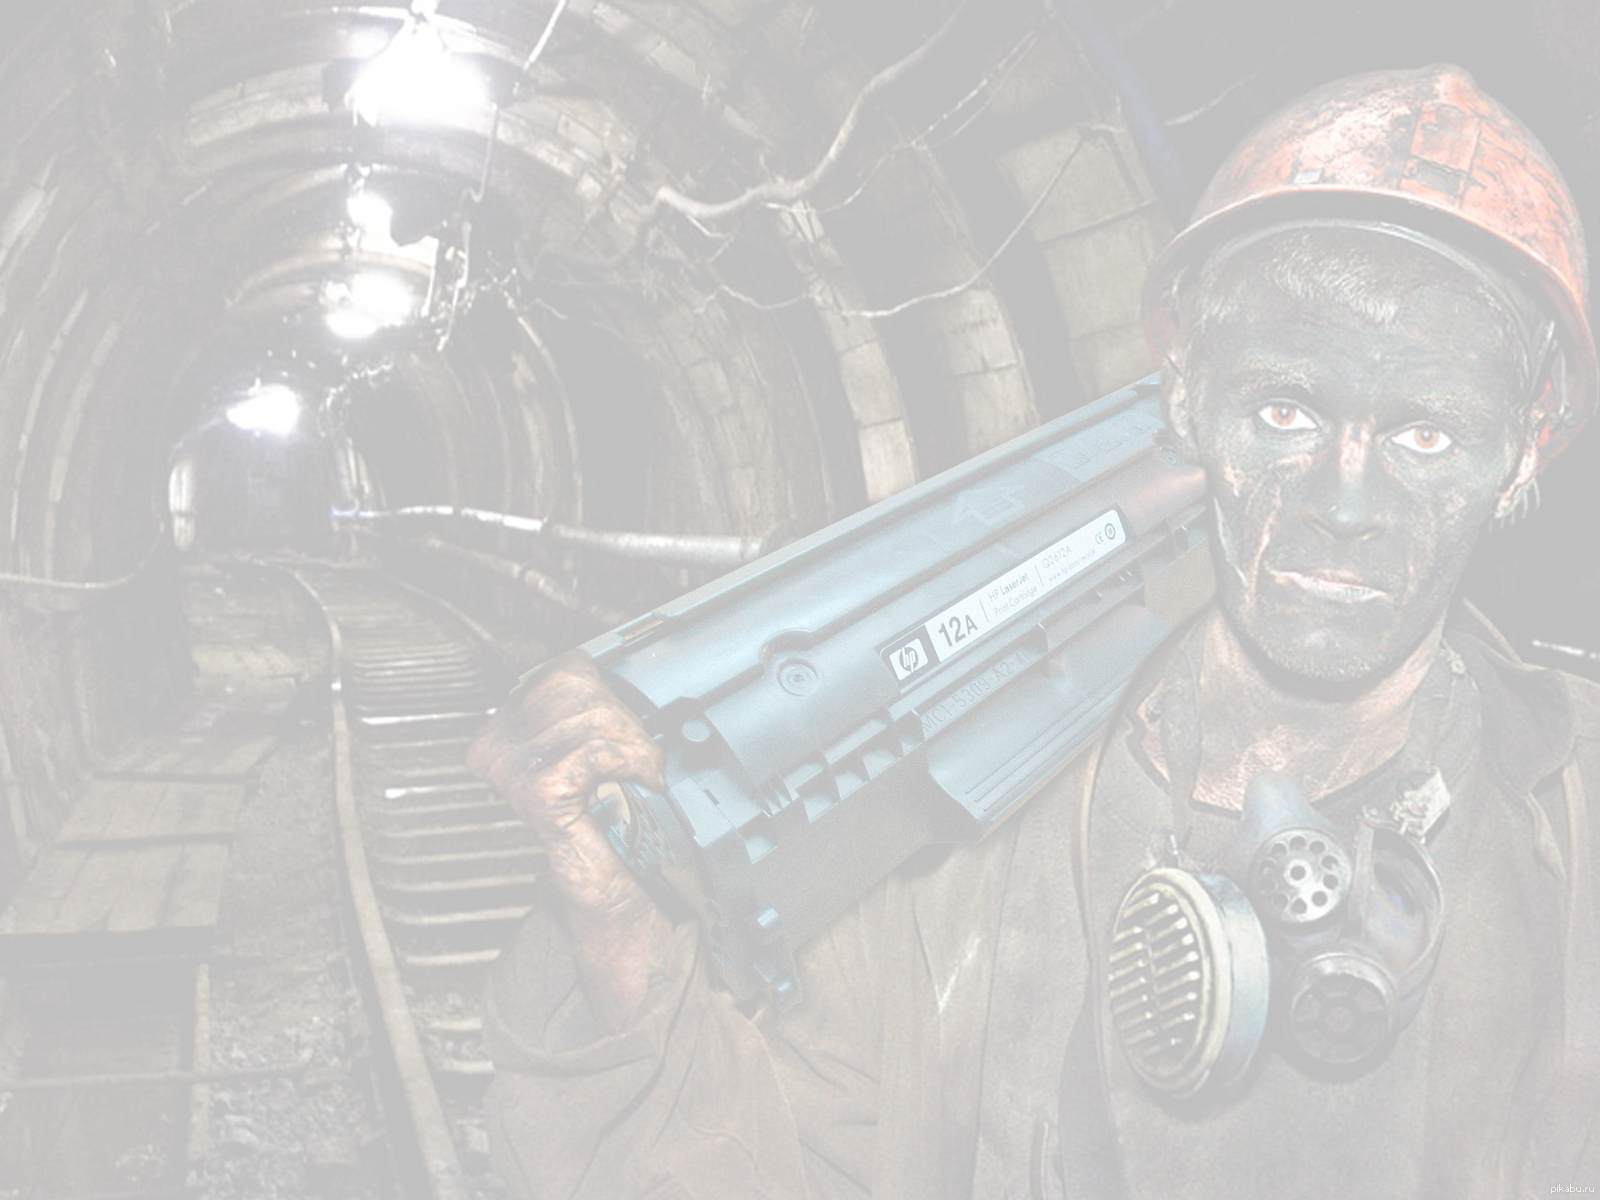
\includegraphics[height=\paperheight,width=\paperwidth]{miner2.jpg}};}
\begin{frame}{Сложности}
\begin{mybox}[]
\begin{itemize}
	\item Можно перенести вручную
	\item Много рутинной работы
	\item Попробовать автоматизировать?
\end{itemize}
\end{mybox}
\end{frame}
}

{
\usebackgroundtemplate{%
\tikz\node[opacity=0.4]{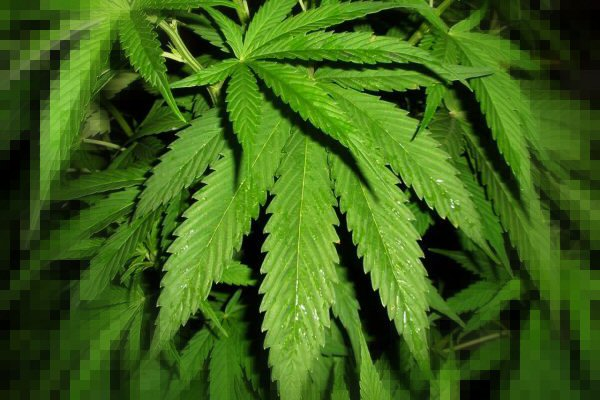
\includegraphics[height=\paperheight,width=\paperwidth]{plan.jpg}};}
\begin{frame}{Общий план решения задачи}
\begin{mybox}[]
\begin{itemize}
	\item Создать модели используемых библиотек
	\item Модель - частная спецификация, описывающая внешнее поведение библиотеки
	\item Найти соответствие между двумя моделями
	\item Преобразовать изменения обратно в код
\end{itemize}
\end{mybox}

\metroset{block=fill}
\begin{alertblock}{Почему модели, а не сам код?}
Не тьюринг-полные модели проще анализировать
\end{alertblock}
\end{frame}
}

\begin{frame}[fragile]{Формализм}
  \begin{mybox}[]
  \begin{itemize}
  	\item Для описания моделей используются расширенные конечные автоматы
  \end{itemize}
  \end{mybox}
\end{frame}

% \section{Titleformats}

\begin{frame}{Пример автомата}
	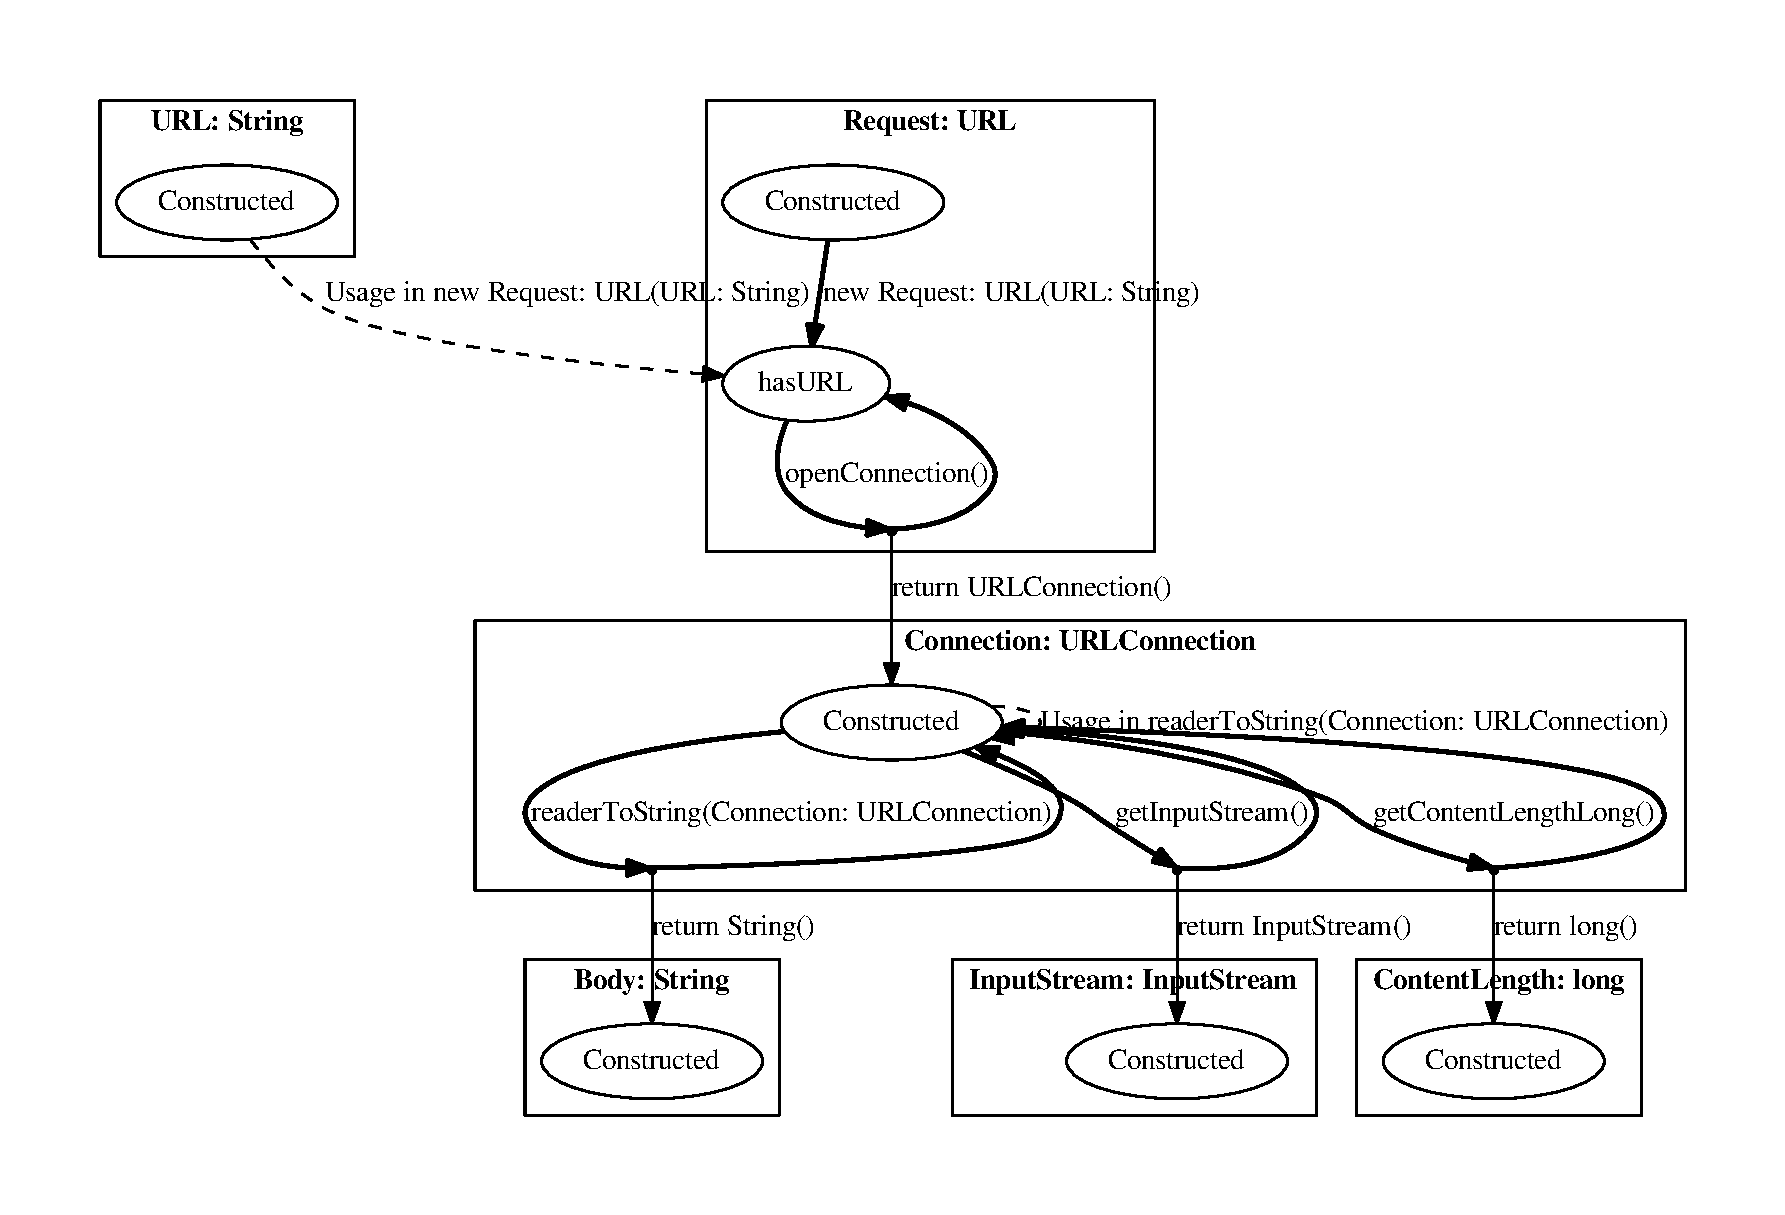
\includegraphics[width=\textwidth]{java.pdf}
\end{frame}

\begin{frame}{Пример автомата}
	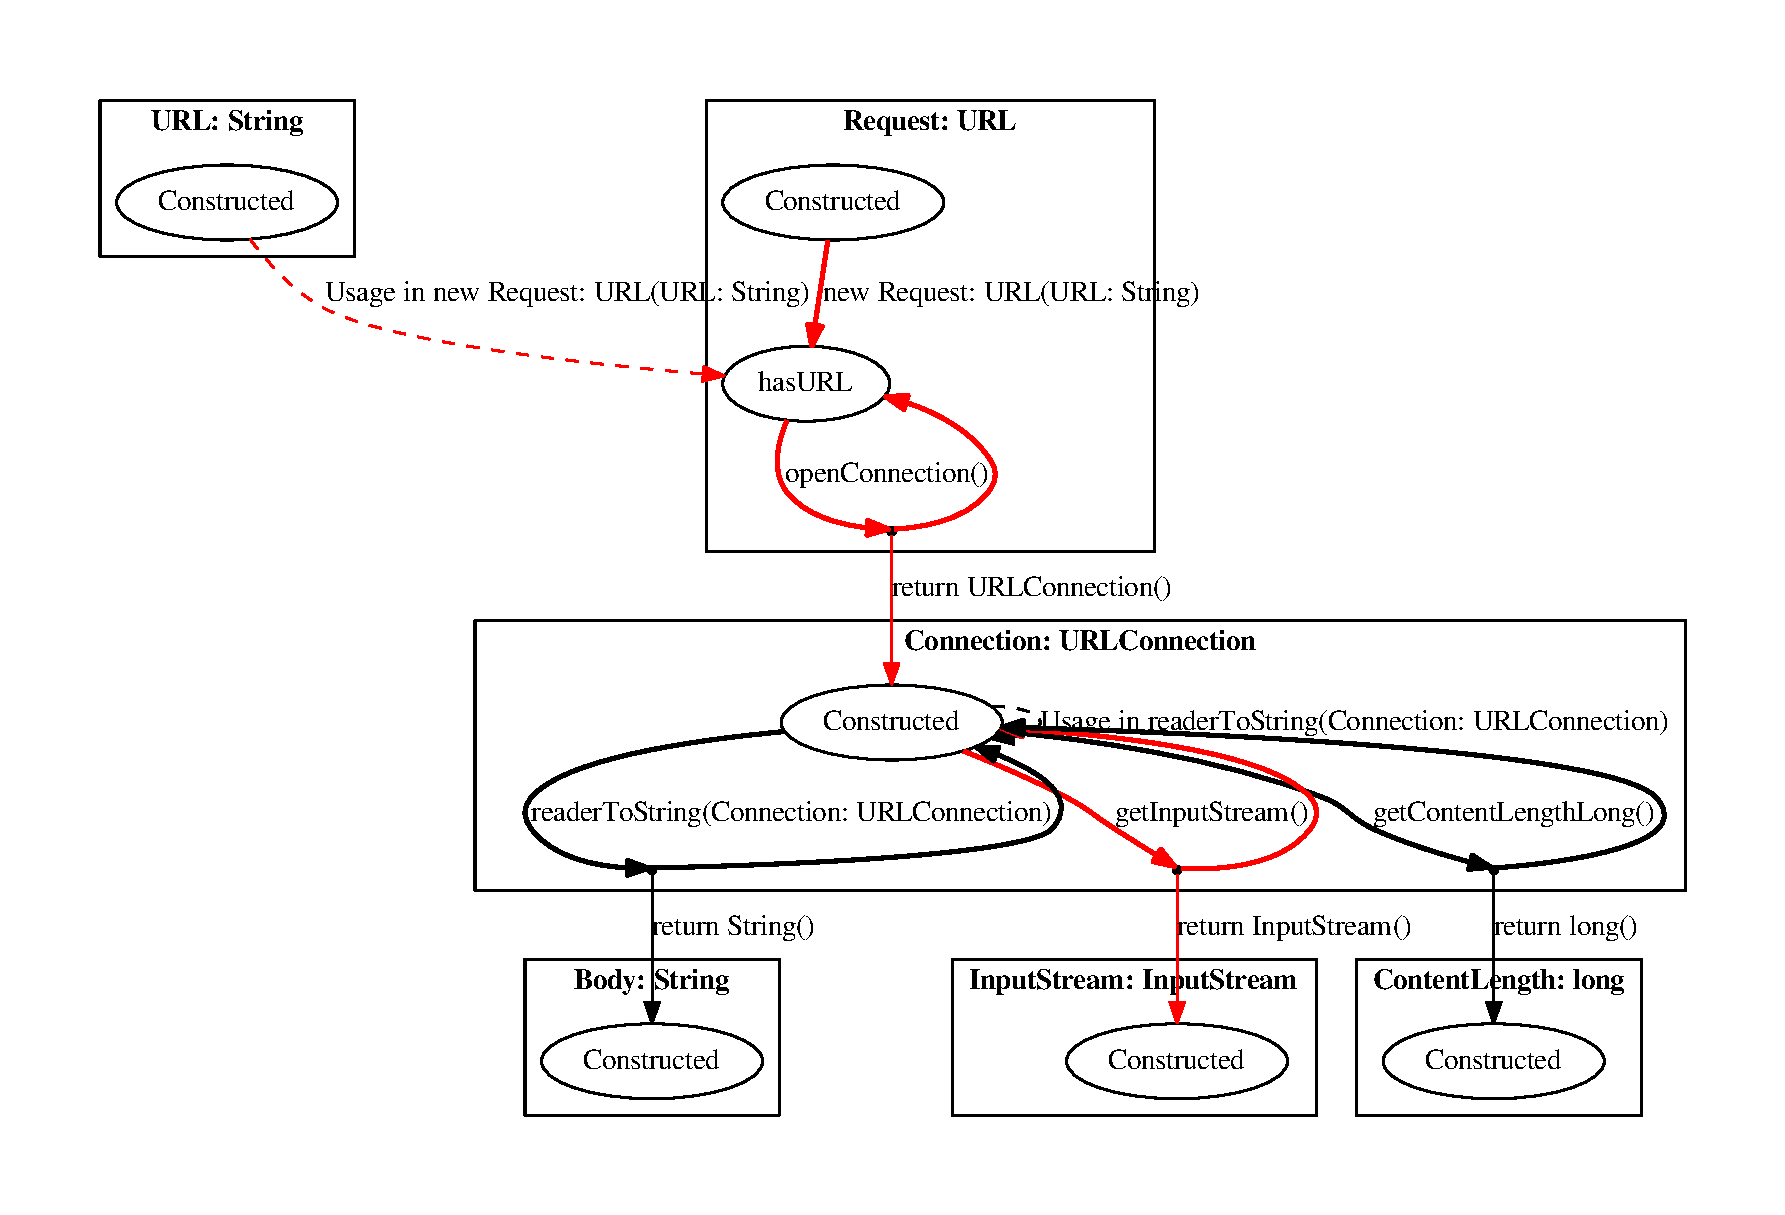
\includegraphics[width=\textwidth]{extracted_java.pdf}
\end{frame}

\begin{frame}[fragile]{Отображение кода на модель}
  \begin{mybox}[]
  \begin{itemize}
  	\item Динамическое отображение: программа инструментируется, на основе трассы выполнения составляется путь в модели
  	\item Для инструментирования используется AOP (аспекты) в реализации AspectJ
  	\item Бонус: проверка корректности использования исходной библиотеки
  \end{itemize}
  \end{mybox}
\end{frame}

\begin{frame}[fragile]{Поиск соответствия между моделями}
  \begin{mybox}[]
  \begin{itemize}
  	\item При переносе необходимо сохранить:
  	  \begin{itemize}
  	  	\item Набор действий, совершенных над библиотекой
  	  	\item Зависимости по данным
  	  \end{itemize}
  	\item Первые версии инструмента: модель преобразуется в граф, с помощью алгоритма Дейкстры ищем кратчайший путь между вершинами
  	\item Сейчас: используется волновой алгоритм
  \end{itemize}
  \end{mybox}
\end{frame}

\begin{frame}[fragile]{Текущее состояние}
  \begin{mybox}[]
  \begin{itemize}
  	\item DSL на базе Kotlin для описания моделей
  	\item Инструмент для миграции программ на языке Java
  	\item Система проверки корректности преобразования
  \end{itemize}
  \end{mybox}
\end{frame}

\begin{frame}[fragile]{Пример миграции}
До:
\begin{lstlisting}
URL url = new URL("http://api.ipify.org/");
URLConnection conn = url.openConnection();
if (conn.getContentLengthLong() > 0) {
    String response = new BufferedReader(new InputStreamReader(conn.getInputStream())).lines().collect(Collectors.joining("\n"));
    System.out.println(response);
} else {
    System.out.println("Error!");
}
\end{lstlisting}
\end{frame}

\begin{frame}[fragile]{Пример миграции}
После:
\begin{lstlisting}
HttpGet url = new HttpGet("http://api.ipify.org/");
CloseableHttpClient newMachine_Client_0 = HttpClients.createDefault();
CloseableHttpResponse conn = newMachine_Client_0.execute(url);
long linkedEdge_ContentLength_1 = conn.getEntity().getContentLength();
if (linkedEdge_ContentLength_1 > 0) {
    InputStream linkedEdge_InputStream_2 = conn.getEntity().getContent();
    String response = new BufferedReader(new InputStreamReader(linkedEdge_InputStream_2)).lines().collect(Collectors.joining("\n"));
    System.out.println(response);
} else {
    System.out.println("Error!");
}
\end{lstlisting}
\end{frame}

{
    \metroset{titleformat frame=smallcaps}
\begin{frame}{Small caps}
	This frame uses the \texttt{smallcaps} titleformat.

	\begin{alertblock}{Potential Problems}
		Be aware, that not every font supports small caps. If for example you typeset your presentation with pdfTeX and the Computer Modern Sans Serif font, every text in smallcaps will be typeset with the Computer Modern Serif font instead.
	\end{alertblock}
\end{frame}
}

{
\metroset{titleformat frame=allsmallcaps}
\begin{frame}{All small caps}
	This frame uses the \texttt{allsmallcaps} titleformat.

	\begin{alertblock}{Potential problems}
		As this titleformat also uses smallcaps you face the same problems as with the \texttt{smallcaps} titleformat. Additionally this format can cause some other problems. Please refer to the documentation if you consider using it.

		As a rule of thumb: Just use it for plaintext-only titles.
	\end{alertblock}
\end{frame}
}

{
\metroset{titleformat frame=allcaps}
\begin{frame}{All caps}
	This frame uses the \texttt{allcaps} titleformat.

	\begin{alertblock}{Potential Problems}
		This titleformat is not as problematic as the \texttt{allsmallcaps} format, but basically suffers from the same deficiencies. So please have a look at the documentation if you want to use it.
	\end{alertblock}
\end{frame}
}

\section{Elements}

\begin{frame}[fragile]{Typography}
      \begin{verbatim}The theme provides sensible defaults to
\emph{emphasize} text, \alert{accent} parts
or show \textbf{bold} results.\end{verbatim}

  \begin{center}becomes\end{center}

  The theme provides sensible defaults to \emph{emphasize} text,
  \alert{accent} parts or show \textbf{bold} results.
\end{frame}

\begin{frame}{Font feature test}
  \begin{itemize}
    \item Regular
    \item \textit{Italic}
    \item \textsc{SmallCaps}
    \item \textbf{Bold}
    \item \textbf{\textit{Bold Italic}}
    \item \textbf{\textsc{Bold SmallCaps}}
    \item \texttt{Monospace}
    \item \texttt{\textit{Monospace Italic}}
    \item \texttt{\textbf{Monospace Bold}}
    \item \texttt{\textbf{\textit{Monospace Bold Italic}}}
  \end{itemize}
\end{frame}

\begin{frame}{Lists}
  \begin{columns}[T,onlytextwidth]
    \column{0.33\textwidth}
      Items
      \begin{itemize}
        \item Milk \item Eggs \item Potatos
      \end{itemize}

    \column{0.33\textwidth}
      Enumerations
      \begin{enumerate}
        \item First, \item Second and \item Last.
      \end{enumerate}

    \column{0.33\textwidth}
      Descriptions
      \begin{description}
        \item[PowerPoint] Meeh. \item[Beamer] Yeeeha.
      \end{description}
  \end{columns}
\end{frame}
\begin{frame}{Animation}
  \begin{itemize}[<+- | alert@+>]
    \item \alert<4>{This is\only<4>{ really} important}
    \item Now this
    \item And now this
  \end{itemize}
\end{frame}
\begin{frame}{Tables}
  \begin{table}
    \caption{Largest cities in the world (source: Wikipedia)}
    \begin{tabular}{lr}
      \toprule
      City & Population\\
      \midrule
      Mexico City & 20,116,842\\
      Shanghai & 19,210,000\\
      Peking & 15,796,450\\
      Istanbul & 14,160,467\\
      \bottomrule
    \end{tabular}
  \end{table}
\end{frame}
\begin{frame}{Blocks}
  Three different block environments are pre-defined and may be styled with an
  optional background color.

  \begin{columns}[T,onlytextwidth]
    \column{0.5\textwidth}
      \begin{block}{Default}
        Block content.
      \end{block}

      \begin{alertblock}{Alert}
        Block content.
      \end{alertblock}

      \begin{exampleblock}{Example}
        Block content.
      \end{exampleblock}

    \column{0.5\textwidth}

      \metroset{block=fill}

      \begin{block}{Default}
        Block content.
      \end{block}

      \begin{alertblock}{Alert}
        Block content.
      \end{alertblock}

      \begin{exampleblock}{Example}
        Block content.
      \end{exampleblock}

  \end{columns}
\end{frame}
\begin{frame}{Math}
  \begin{equation*}
    e = \lim_{n\to \infty} \left(1 + \frac{1}{n}\right)^n
  \end{equation*}
\end{frame}
\begin{frame}{Line plots}
\end{frame}
\begin{frame}{Bar charts}
\end{frame}
\begin{frame}{Quotes}
  \begin{quote}
    Veni, Vidi, Vici
  \end{quote}
\end{frame}

\begin{frame}{References}
  Some references to showcase [allowframebreaks] \cite{knuth92,ConcreteMath,Simpson,Er01,greenwade93}
\end{frame}

\section{Conclusion}

\begin{frame}{Summary}

  Get the source of this theme and the demo presentation from

  \begin{center}\url{github.com/matze/mtheme}\end{center}

  The theme \emph{itself} is licensed under a
  \href{http://creativecommons.org/licenses/by-sa/4.0/}{Creative Commons
  Attribution-ShareAlike 4.0 International License}.

\end{frame}

\begin{frame}[standout]
  Questions?
\end{frame}

\appendix

\begin{frame}[fragile]{Backup slides}
  Sometimes, it is useful to add slides at the end of your presentation to
  refer to during audience questions.

  The best way to do this is to include the \verb|appendixnumberbeamer|
  package in your preamble and call \verb|\appendix| before your backup slides.

  \themename will automatically turn off slide numbering and progress bars for
  slides in the appendix.
\end{frame}

\begin{frame}[allowframebreaks]{References}

  \bibliography{demo}
  \bibliographystyle{abbrv}

\end{frame}

\end{document}
